\documentclass[french]{beamer}

\usepackage[T1]{fontenc}
\usepackage[french]{babel}
\usepackage{physics} % \bra et \ket

\usepackage{amsmath}
\usepackage{amsfonts}
\newcommand{\somme}{\displaystyle\sum}

\usetheme{Berlin}
\beamertemplatenavigationsymbolsempty
\setbeamertemplate{footline}[fame number]

\usepackage{graphicx}
\graphicspath{ {./Images/} }

\usepackage{tikz}
\usetikzlibrary{positioning}

\title{De la quantique en cryptographie}
\author{Élie Besnard, Malo Leroy, \\
Yun Marcola--da-Cunha Macedo}
\institute{Lycée Chateaubriand}


\begin{document}


\section{Introduction}

\begin{frame}
\titlepage
\end{frame}


\begin{frame}{Motivation}
\begin{itemize}
    \item<1-> Qu'est-ce que la cryptographie ?
    \item<2> Ancrage au thème
\end{itemize}
\end{frame}


\section{Calcul quantique}


\subsection{Modèle du cicruit quantique}


\begin{frame}{Un exemple}
    % Exemple de circuit simple
    % Comparaison avec les circuits électriques
    \begin{center}
        \begin{tikzpicture}[
            node distance=0.1 cm and 1cm,
            porte/.style={rectangle, draw=black},
            swap/.style={rectangle, draw=black, minimum height=1.8cm},]
            % Nœuds du circuit
            \node          (ei1)    at (0, 1)     {$\ket{\psi_{i, 0}}$};
            \node          (ei2)    at (0, 0)     {$\ket{\psi_{i, 1}}$};
            \node[swap]    (s1)     at (1, 0.5)   {S};
            \node          (x1)     at (2, 1)     {$\oplus$};
            \node[swap]    (s2)     at (3, 0.5)   {S};
            \node          (x2)     at (4, 0)     {$\oplus$};
            \node          (ef1)    at (5, 1)     {$\ket{\psi_{f, 0}}$};
            \node          (ef2)    at (5, 0)     {$\ket{\psi_{f, 1}}$};
            % Arrêtes
            \draw (0.5, 1)       -- (0.77, 1);
            \draw (0.5, 0)       -- (0.77, 0);
            \draw (1.23, 1)      -- (2.77, 1);
            \draw (1.23, 0)      -- (2.77, 0);
            \draw (3.23, 1)      -- (4.5, 1);
            \draw (3.23, 0)      -- (4.5, 0);
        \end{tikzpicture}
    \end{center}
    $$S \cdot (X \otimes I_2) \cdot (I_2 \otimes X) \cdot S = I_4$$
    % \underline{Application :} test de parité
\end{frame}


\subsection{Calcul formel}


\begin{frame}{Calcul formel}
    \begin{itemize}
        \item<1-> Valeurs exactes : $\frac 2 5, \sqrt 2, e^{\frac{i\pi}{7}}, \pi + 3^{2/3}$, etc.
            % nécessité, cf. Shor
            % valeurs très diverses
        \item<2-> Produit de Kronecker, produit matriciel, etc.
        \item<3-> Efficacité algorithmique
            % complexité sur-exponentielle
            % analyses de complexité
    \end{itemize}
\end{frame}

\subsection{Algorithmes}


\begin{frame}{Deutsch-Jozsa et Bernstein-Vazirani}
    % Explication de l'algorithme: pièces
    % Interface graphique
    \begin{columns}
        \begin{column}{0.5\textwidth}
            \begin{tikzpicture}[
                node distance=0.3cm and 1cm,
                porte/.style={rectangle, draw=black},
                oracle/.style={fill=white, rectangle, draw=black, minimum height=2.6cm},]
                % Nœuds du circuit
                \node              (e0)                        {$\ket 0$};
                \node              (p_ei)   [below=of e0]      {$\vdots$};
                \node              (e1)     [below=of p_ei]    {$\ket 0$};
                \node[porte]       (hi0)    [right=of e0]      {H};
                \node              (p_hi)   [right=of p_ei]    {$\vdots$};
                \node[porte]       (hi1)    [right=of e1]      {H};
                \node[porte]       (hf0)    [right=2cm of hi0] {H};
                \node              (p_hf)   [below=of hf0]     {$\vdots$};
                \node[porte]       (hf1)    [right=2cm of hi1] {H};
                % Arrêtes
                \draw (e0.east)    -- (hi0);
                \draw (e1.east)    -- (hi1);
                \draw (hi0.east)   -- (hf0);
                \draw (hi1.east)   -- (hf1);
                \node[oracle]      (uf)     [right=of p_hi]    {$U_f$};
                % \draw (uf)         -- (hf0);
                % \draw (uf)         -- (hf1);
            \end{tikzpicture}
        \end{column}
        \begin{column}{0.5\textwidth}
            \underline{Exemples :} oracles
            \begin{itemize}
                \item de phase $U_f \ket x = (-1)^{f(x)} \ket x$
                \item par somme $U_f \ket{x, y} = \ket{x, y \oplus f(y)}$
            \end{itemize}
        \end{column}
    \end{columns}
    \vspace{1em}
    \underline{Application :} Bernstein-Vazirani,
    $f(x_1, ..., x_n) = \somme_{i=0}^n x_i \cdot a_i \in \mathbb{F}_2$
\end{frame}


\begin{frame}{Shor}
    % Explication de l'algorithme
    \begin{center}
        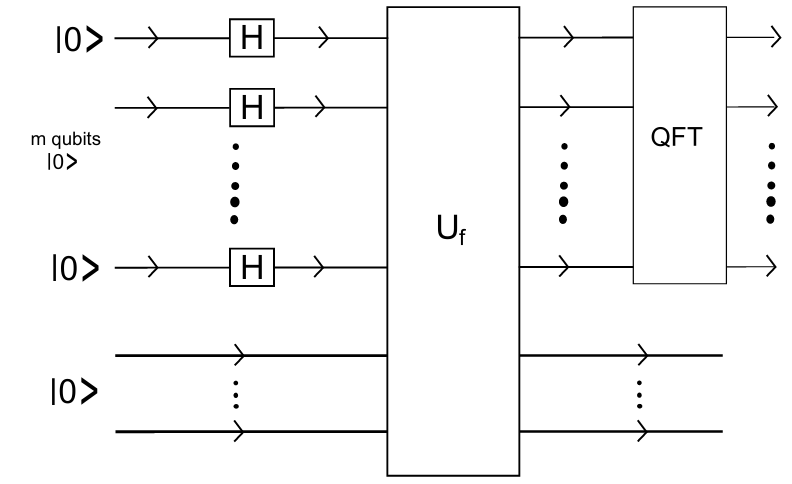
\includegraphics[scale=0.25]{Fabrice.png}
    \end{center}
    \underline{Exemple :} % IBM
\end{frame}


\begin{frame}{Grover}
    % Explication de l'algorithme
\end{frame}

\begin{frame}{Interface graphique}
    % ...
\end{frame}

\section{Cryptographie quantique}

\begin{frame}{Cryptographie quantique}
\begin{itemize}
    \item<1-> Le protocole E91
    \begin{itemize}
        \item Expérience
        \item Simulation
    \end{itemize}
    \item<2-> Tentative de création d'un protocole
\end{itemize}
\end{frame}

\end{document}
